\section{Novelty Search}
Section \ref{sec:novelty} describes how CA-NEAT was extended to support novelty search.

Because novelty search disregards the objective,
a search for a specific neighborhood size $N$ and number of states $K$ creates population that can be used on any CA with that $N$ or $K$.
For example, the same population could contain solutions to both morphogenesis and replication of both the 6x6 "Tricolor" and 7x7 "Nordic" patterns (Figure \ref{fig:patterns}).

\subsection{Results}
\begin{figure}
\centering
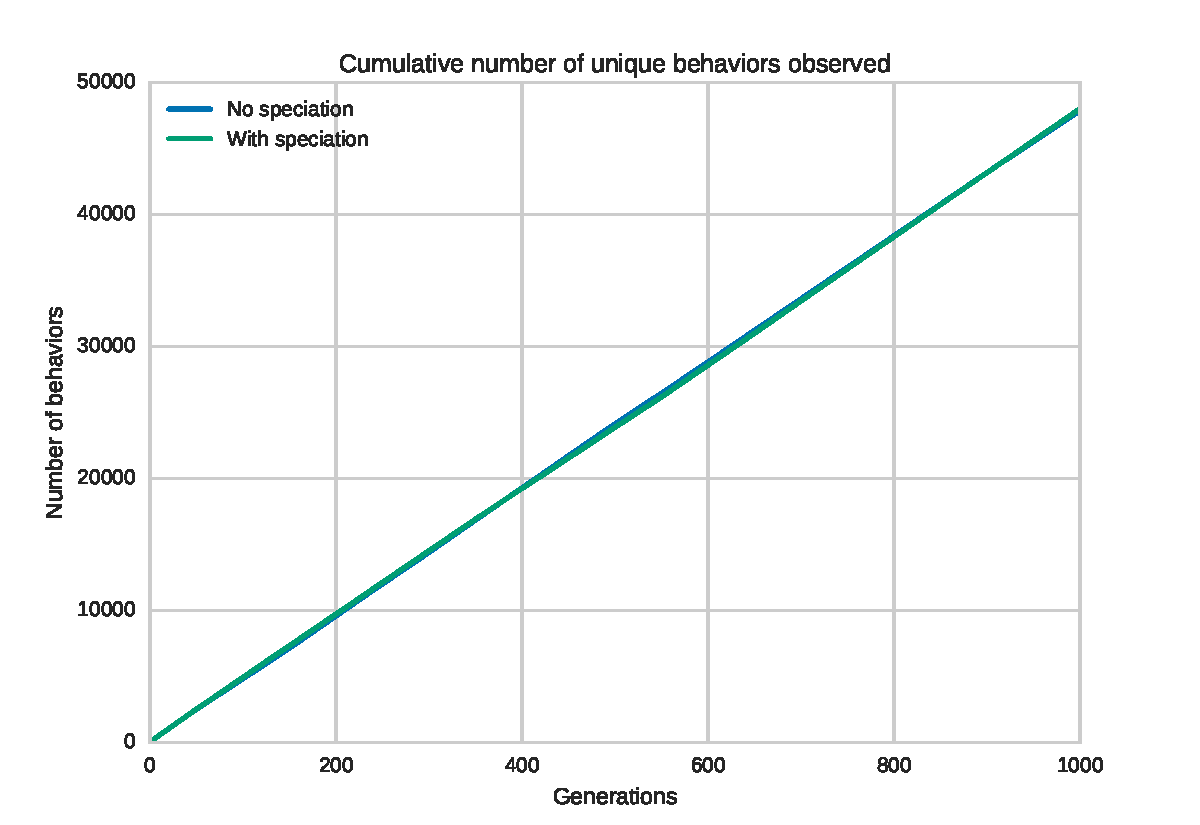
\includegraphics[height=0.4\textheight, width=\textwidth, keepaspectratio]{fig/novelty_diversity}
\caption[
    Cumulative number of unique behaviors observed
]{
    Cumulative number of unique behaviors observed.
    The two runs share the properties $N=5, K=4, P=50, G=1000$, and differ in whether they have speciation enabled.
}
\label{fig:novelty_diversity}
\end{figure}

\begin{figure}
\centering
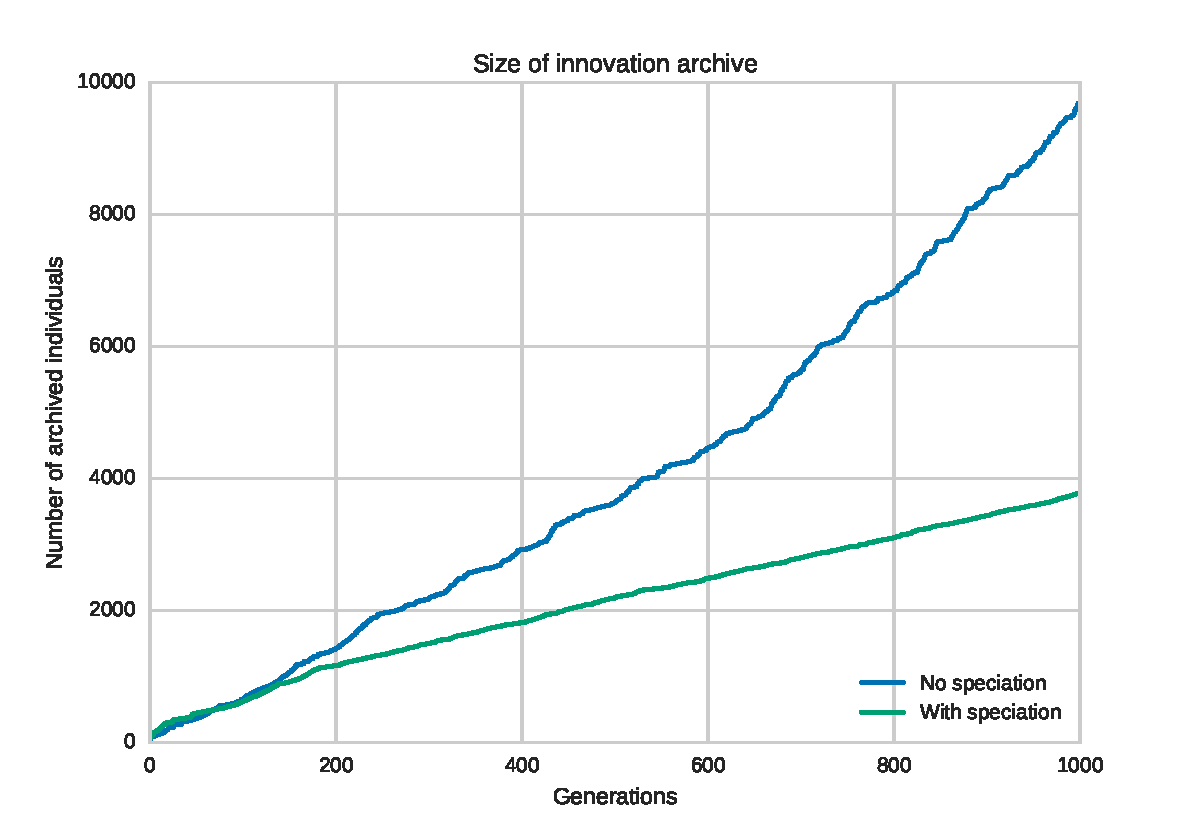
\includegraphics[height=0.4\textheight, width=\textwidth, keepaspectratio]{fig/innovation_archive_size}
\caption[
    Size of the innovation archives
]{
    Size of the innovation archives.
    The archives are a subset of their corresponding populations.
}
\label{fig:innovation_archive_size}
\end{figure}

\begin{table}
\centering
\caption{Overview of the novelty search runs attempted}
\begin{tabular}{c|c|c|c|c|l}
    N   &   K   &   P   &   G   &   Speciation  &   Objectives tested   \\\hline
    5   &   4   &   50  &   1000    &   Yes &   \{Swiss, Nordic\} \{morphogenesis, replication\} \\
    5   &   4   &   50  &   1000    &   No  &   \{Swiss, Nordic\} \{morphogenesis, replication\} \\
    5   &   2   &   50  &   1000    &   No  &   Border morphogenesis \\
    7   &   2   &   200 &   1000    &   No  &   Majority, synchronization
\end{tabular}
\label{tbl:novelty}
\end{table}

Several different $N$ and $K$ combinations were tested and the resulting innovations archives checked against the objective function of appropriate tasks.
Table \ref{tbl:novelty} gives an overview of the combinations tested.
When testing against the appropriate objective functions, the results were not particularly useful, with no optimal solutions found for any of the tasks tested.
Detailed results about the fitnesses found are not too interesting and is omitted from this report.
Suffice it to say, the success rate was 0\% across the board.

One configuration that was tested was $N=5$, $K=4$, a population size of $P=50$, for $G=1000$ generations.
We will take closer look at the results, assuming them to be representative for the results of all the experiments.
This configuration was tested in two independent runs, with and without speciation.
Figure \ref{fig:novelty_diversity} shows the cumulative number of unique behaviors observed in the two runs.
The figure is created from the full population of each run, not the innovation archive, which is a subset of the full population.
It shows that the novelty search is correctly implemented and does in fact produce many novel genotypes in each generation.
It can be compared to Figure \ref{fig:cummulative_unique_behaviors} in Section \ref{sec:properties}, taking into account the different population size
The curves are approximately equal, showing no particular effect from the presence or lack of speciation.
At 1000 generations, the runs are at 47806 unique individuals (no speciation) and 47969 (with speciation).
This is as good as equal, and it is close to the curve of the maximum possible unique behaviors $y(x)=50x$.
Still, $50000$ unique individuals would still only be $\frac{50000}{2^{2^{5}}} \approx 0.0012\%$ of the search space.

Figure \ref{fig:innovation_archive_size} shows the development of the sizes of the innovation archives.
The two archive sizes are approximately the same in the first 150 generations, but then diverge considerably.
The population without speciation adds much fewer innovations to the archive than the population with speciation does.
Over 1000 generations, the population with speciation adds on average almost 10 individuals to the archive per generation,
while the population with speciation adds on average 3-4 innovations per generation.
Since the speciation threshold is supposed to dynamically adjust to keep the number of added innovations between 1-5,
this must mean that the average innovation metric in the population is changing a lot, so that the threshold is not able to keep up.
This could happen because the average innovation degree is continuously increasing, or because it is fluctuating around some value.
In either case the threshold adjusting algorithm is always a step behind.

Because of performance issues with the implementation,
it was not feasible to run many independent trials of the same configuration.
There is a possibility that in a larger number of trials, some might succeed.
But a more performant implementation is necessary to test this.

These results suggest that this approach to novelty search is not going to lead to produce anything that is more interesting than what objective search produces.
This does not necessarily mean that novelty search is never going to work for CA problems, only that the setup used in these experiments is flawed and must be reconsidered.
